% The main file for CAMP reports
% Don't put any content in here.
% Don't even include content files by using \input or \inlcude.
% Put your content to TEXT.TEX or include it there using \input.
% Uses:
%		SETTINGS.TEX	contains the settings for this document
%		COMMANDS.TEX	contains commands which can be used while writing
%		INFO.TEX			contains the author, title and so on for the cover
%		COVER.TEX			formats the front cover of the document
%		ABSTRACT.TEX	contains the abstract to be included (if needed)
%		TEXT.TEX			contains the actual content of the document
%		BIB.BIB				containt the BibTeX entries for the document


%% Draft document mode
%% Final document
\documentclass[11pt,a4paper,biblography=totoc,index=totoc,headsepline,footsepline,footinlcude=false,BCOR12mm,DIV13]{scrbook}

%\documentclass[11pt,a4paper,bibtotoc,idxtotoc,headsepline,footsepline,footexclude,BCOR20mm,DIV10]{scrbook}

% KOMA-Optionen:
%  bibtotoc: include bibliography in table of contents
%  idxtotoc: include index in table of contents
%  headsepline: use horizontal line under heading
%  BCOR: binding correction (Bindungskorrektur) (e.g.: BCOR5mm)
%  DIV: Number of sheet sections (used for layout) (e.g.: DIV12)



% include title and author information for the cover
% Set here the title, authors and other stuff to be used for the cover
% This file is used by MAIN.TEX

% set title, authors and stuff for the cover
\def\doctype{Master's Thesis}
\def\title{A Practical Approach to Walking on Spheres with GPUs}
\def\author{Walter Arthur Simson IV}
\def\examinerOne{Prof. Dr. Folkmar Bornemann}
\def\examinerTwo{Univ.-Prof. Dr. Thomas Huckle}

\def\date{April 1, 2017}

% text to appear in the footer
\def\footertext{}


% include settings
% Included by MAIN.TEX
% Defines the settings for the CAMP report document

\renewcommand{\sectfont}{\normalfont \bfseries}        % Schriftart der Kopfzeile

% manipulate footer
\usepackage{scrpage2}
\pagestyle{scrheadings}
\ifoot[\footertext]{\footertext} % \footertext set in INFO.TEX
%\setkomafont{pagehead}{\normalfont\rmfamily}
\setkomafont{pagenumber}{\normalfont\rmfamily}

%% allow sophisticated control structures
\usepackage{ifthen}

% use Palatino as default font
\usepackage{palatino}

% enable special PostScript fonts
\usepackage{pifont}

% make thumbnails
% \usepackage{thumbpdf}

%to use the subfigures
\usepackage{subfigure}


\usepackage{colortbl}

\usepackage{multicol}

\usepackage{commath}

\usepackage{algorithm}
\usepackage{algpseudocode}
%black tirangle comments
% \algrenewcommand{\algorithmiccomment}[1]{\hfill$\blacktriangleright$ #1}
%normal arrow comments
\algrenewcommand{\algorithmiccomment}[1]{\hfill$\rightarrow$ #1}

%% show program code\ldots
%\usepackage{verbatim}
%\usepackage{program}

%% enable TUM symbols on title page
\usepackage{styles/tumlogo}


\usepackage{multirow}

%% use colors
\usepackage{color}

%% make fancy math
\usepackage{amsmath}
\usepackage{amsfonts}
\usepackage{amssymb}
\usepackage{textcomp}
\usepackage{yhmath} % fr die adots
%% mark text as preliminary

%% create an index
\usepackage{makeidx}

% for the program environment
\usepackage{float}
%for glossary
\usepackage[toc,  xindy]{glossaries}

%% load german babel package for german abstract
%\usepackage[german,american]{babel}
\usepackage[german,english]{babel}
\selectlanguage{english}

% use german characters as well
\usepackage[latin1]{inputenc}       % allow Latin1 characters

% use initals dropped caps - doesn't work with PDF
%\usepackage{dropping}
 %\usepackage[dvips]{dropping}

\usepackage{styles/shortoverview}
%----------------------------------------------------
%      Graphics and Hyperlinks
%----------------------------------------------------

%% check for pdfTeX
\ifx\pdftexversion\undefined
 %% use PostScript graphics
 \usepackage[dvips]{graphicx}

 \DeclareGraphicsExtensions{.eps,.epsi}
 \graphicspath{{figures/}{figures/review}}
 %% allow rotations
 \usepackage{rotating}
 %% mark pages as draft copies
 %\usepackage[english,all,light]{draftcopy}
 %% use hypertex version of hyperref
 \usepackage[hypertex,hyperindex=false,colorlinks=false]{hyperref}
\else %% reduce output size \pdfcompresslevel=9
 %% declare pdfinfo
 %\pdfinfo {
 %  /Title (my title)
 %  /Creator (pdfLaTeX)
 %  /Author (my name)
 %  /Subject (my subject	)
 %  /Keywords (my keywords)
 %}
 %% use pdf or jpg graphics
 \usepackage[pdftex]{graphicx}
 \DeclareGraphicsExtensions{.jpg,.JPG,.png,.pdf,.eps}
 \graphicspath{{figures/}}

 %% Load float package, for enabling floating extensions
 \usepackage{float}

 %% allow rotations
 \usepackage{rotating}
 %% use pdftex version of hyperref
 \usepackage[pdftex,colorlinks=true,linkcolor=red,citecolor=red,%
 anchorcolor=red,urlcolor=red,bookmarks=true,%
 bookmarksopen=true,bookmarksopenlevel=0,plainpages=false%
 bookmarksnumbered=true,hyperindex=false,pdfstartview=%
 ]{hyperref}
\fi




%% Fancy chapters
%\usepackage[Lenny]{fncychap}
%\usepackage[Glenn]{fncychap}
%\usepackage[Bjarne]{fncychap}

%\usepackage[avantgarde]{quotchap}

% set the bibliography style
%\bibliographystyle{styles/bauermaNum}
%\bibliographystyle{alpha}
\bibliographystyle{plain}


% include commands
% Commands to be used within the TUM report document
% Included by MAIN.TEX
% Please include your own cool commands here. 
% Be only sure to comment it sufficiently so others can use it.

%-------------------------------------------------------------
%                      Own Commands
%-------------------------------------------------------------


%-------------------------------------------------------------
% math stuff -------------------------------------------------

% nice R, N, C
\newcommand{\nat}{\mathbb{N}}
\newcommand{\real}{\mathbb{R}}
\newcommand{\compl}{\mathbb{C}}



% norm
\newcommand{\norm}[1]{\left\| #1 \right\|}

% un demi
\newcommand{\half}{\frac{1}{2}}

% parantheses
\newcommand{\parenth}[1]{ \left( #1 \right) }
\newcommand{\bracket}[1]{ \left[ #1 \right] }
\newcommand{\accolade}[1]{ \left\{ #1 \right\} }
%\newcommand{\angle}[1]{ \left\langle  #1 \right\rangle }

% partial derivative: %#1 function, #2 which variable
% simple / single line version
\newcommand{\pardevS}[2]{ \delta_{#1} f(#2) }
% fraction version
\newcommand{\pardevF}[2]{ \frac{\partial #1}{\partial #2} }

% render vectors: 3 and 4 dimensional
\newcommand{\veciii}[3]{\left[ \begin{array}[h]{c} #1 \\ #2 \\ #3	\end{array} \right]}
\newcommand{\veciv}[4]{\left[ \begin{array}[h]{c} #1 \\ #2 \\ #3 \\ #4	\end{array} \right]}

% render matrices: 3  dimensional (arguments in row first order)
\newcommand{\matiii}[9]{\left[ \begin{array}[h]{ccc} #1 & #2 & #3 \\ #4 & #5 & #6 \\ #7 & #8 & #9	\end{array} \right]}
%DOESN'T WORK,DON'T KNOW WHY \newcommand{\mativ}[16]{\left[ \begin{array}[h]{cccc} #1 & #2 & #3 & #4 \\ #5 & #6 & #7 & #8 \\ #9 & #10 & #11 & #12 \\ #13 & #14 & #15 & #16 \end{array} \right]}


%-------------------------------------------------------------
%-------------------------------------------------------------


%-------------------------------------------------------------
% some abreviations ------------------------------------------
\newcommand{\Reg}{$^{\textregistered}$}
\newcommand{\reg}{$^{\textregistered}$ }
\newcommand{\Tm}{\texttrademark}
\newcommand{\tm}{\texttrademark~}
\newcommand {\bsl} {$\backslash$}

%-------------------------------------------------------------
%-------------------------------------------------------------


%-------------------------------------------------------------
% formating --------------------------------------------------

% Theorem & Co environments and counters
\newtheorem{theorem}{Theorem}[chapter]
\newtheorem{lemma}[theorem]{Lemma}
\newtheorem{corollary}[theorem]{Corollary}
\newtheorem{remark}[theorem]{Remark}
\newtheorem{definition}[theorem]{Definition}
\newtheorem{equat}[theorem]{Equation}
\newtheorem{example}[theorem]{Example}
\newtheorem{algorithm}[theorem]{Algorithm}

% inserting figures
\newcommand{\insertfigure}[4]{ % Filename, Caption, Label, Width percent of textwidth
	\begin{figure}[htbp]
		\begin{center}
			\includegraphics[width=#4\textwidth]{#1}
		\end{center}
		\vspace{-0.4cm}
		\caption{#2}
		\label{#3}
	\end{figure}
}




% referecing figures

\newcommand{\refFigure}[1]{ %label
	figure \ref{#1}
}
\newcommand{\refChapter}[1]{ %label
	chapter \ref{#1}
}

\newcommand{\refSection}[1]{ %label
	section \ref{#1}
}

\newcommand{\refParagraph}[1]{ %label
	paragraph \ref{#1}
}

\newcommand{\refEquation}[1]{ %label
	equation \ref{#1}
}

\newcommand{\refTable}[1]{ %label
	table \ref{#1}
}




\newcommand{\rigidTransform}[2]
{
	${}^{#2}\!\mathbf{H}_{#1}$
}

%code, in typewriter
\newcommand{\code}[1]
 {\texttt{#1}}

% comment that appears on the border - very practical !!!
\newcommand{\comment}[1]{\marginpar{\raggedright \noindent \footnotesize {\sl #1} }}

% page clearing
\newcommand{\clearemptydoublepage}{%
  \ifthenelse{\boolean{@twoside}}{\newpage{\pagestyle{empty}\cleardoublepage}}%
  {\clearpage}}


%-------------------------------------------------------------
%-------------------------------------------------------------


\newcommand{\etAl}{\emph{et al.}\mbox{ }}

%include glossary
\newglossaryentry{computer}
{
  name=computer,
  description={is a programmable machine that receives input,
               stores and manipulates data, and provides
               output in a useful format}
}

\newglossaryentry{poc}
{
  name={proof of concept},
  description={}
  }
\newglossaryentry{ui}
{
  name={user interface},
  description={}
  }
\newglossaryentry{ai}
{
  name={arithmetic intensity},
  description={a measure of floating-point operations (FLOPs)
              \hyphenation{per-formed} performed by a \hyphenation{gi-ven} given code or code section relative
              to the amount of memory accesses (Bytes) that are required
               to support those operations\cite{AI}}
  }

\newglossaryentry{speed-up}
{
  name={speed-up},
  description={the factor of temporal acceleration a program
  exhibits when additional computational resources are dedicated to it's execution.}
}

\newglossaryentry{directive pragmas}
{
  name={directive pragma},
  description={a computer programming language construct that specifies how a compiler
  should process input data} % sourced from wikipedia
}


\newglossaryentry{rc}{%SOURCE: wikipedia
name={race condition},
description={A race condition or race hazard is the behavior of an electronic,
 software, or other system where the output is dependent on the sequence or
 timing of other uncontrollable events. It becomes a bug when events do not
 happen in the order the programmer intended. The term originates with the idea
 of two signals racing each other to influence the output first.}
}
\newglossaryentry{dd}{
name={data dependencies},
description={}
}
\newglossaryentry{sisd}{
name={single instruction single data},
description={}
}
\newglossaryentry{simt}{
name={single instruction multiple threads},
description={}
}

\newglossaryentry{simd}{
name={single instruction multiple data},
description={}
}
\newglossaryentry{gp}{%SOURCE: wikipedia
name={Gaussian Plane},
description={The two dimensional plane of complex numbers.}
}
\newglossaryentry{CURAND}{
name={CURAND},
description={
The CURAND library provides facilities that focus on the simple and efficient
generation of high-quality pseudorandom and quasirandom numbers.\cite{cuRAND}
}
}

\newacronym[longplural={partial differential equations}]{PDE}{PDE}{partial differential equations}
\newacronym{mpi}{MPI}{Message Passing Interface}

\newacronym[longplural={Random Walks on Spheres}]{RWoS}{RWoS}{Random Walk on Spheres}

\newacronym[longplural={Graphical Processing Units}]{GPU}{GPU}{Graphical Processing Unit}

\newacronym[longplural={Central Processing Units}]{CPU}{CPU}{Central Processing Unit}
\newacronym{hpc}{HPC}{high performance computing}

\newacronym[longplural={Arithmetic Logic Units}]{ALU}{ALU}{Arithmetic Logic Unit}

\newacronym[longplural={Streaming Multi-Processors}]{SM}{SM}{Streaming Multi-Processor}

\newacronym[longplural={boundary value problems}]{BVP}{BVP}{boundary value problem}
\newacronym[longplural={general purpose graphical processing units}]{GPGPU}{GPGPU}{general purpose graphical processing units}
\newacronym{CUDA}{CUDA}{Compute Unified Device Architecture}
\newacronym{RAM}{RAM}{Random Access Memory}
\newacronym{SRAM}{SRAM}{Static Random Access Memory}
\newacronym{DRAM}{DRAM}{Dynamic Random Access Memory}
\newacronym{I/O}{I/O}{Input/Output}
\newacronym{PTX}{PTX}{Parallel Thread eXecution}
\newacronym{jit}{JIT}{just in time}


%\makeindex
 %% inter line spacing
%\linespread{1.0}

\makeglossary

\begin{document}

 \frontmatter



 %% The front cover for the TUM report document.
% Included by MAIN.TEX


%--------------------------------------------------
% The Front Cover
%--------------------------------------------------

% The front cover for the TUM document.
% Included by MAIN.TEX


%--------------------------------------------------
% The Front Cover
%--------------------------------------------------

% correct BCOR - undo at the end !!!
\def\bcorcor{0.15cm}
\addtolength{\hoffset}{\bcorcor}

\thispagestyle{empty}

 \vspace{4cm}
\begin{center}
	       %\oTUM{4cm}
	       
	  
\includegraphics[width=4cm]{styles/tum_logo.png}
	   
	   \vspace{5mm}     
	   \huge Computational Science and Engineering \\(Int. Master's Program)\\ 
	   \vspace{0.5cm}
	 \large Technische Universit{\"a}t M{\"u}nchen\\
    \vspace{1mm}
        
	\end{center}
		

\vspace{15mm}
\begin{center}

   {\Large \doctype}

  \vspace{20mm}
  
  {\huge\bf \title}\\%[3ex]
  
  
  \vspace{15mm}
  
  
  {\LARGE  \author}
  
  \vspace{10mm}
  
  \begin{figure}[h!]
  \centering
   
\includegraphics[width=4cm]{styles/cse_logo.jpg}
  \end{figure}
  
  \end{center}
%	\clearemptydoublepage
%
%	% The titlepage for the CAMP report document.
% Included by MAIN.TEX


%--------------------------------------------------
% The title page
%--------------------------------------------------

% correct BCOR - undo at the end !!!
\def\bcorcor{0.15cm}
\addtolength{\hoffset}{\bcorcor}

\thispagestyle{empty}

 \vspace{10mm}
\begin{center}
	       %\oTUM{4cm}
	       
\includegraphics[width=4cm]{styles/tum_logo.png}

	   \vspace{5mm}
	   \huge Computational Science and Engineering \\(Int. Master's Program)\\
	   \vspace{0.5cm}
	 \large Technische Universit{\"a}t M{\"u}nchen\\

	\end{center}


\vspace{10mm}
\begin{center}

   {\Large \doctype}

  \vspace{10mm}

  {\LARGE \title}\\


  \vspace{10mm}


  %{\LARGE  \titleGer}\\


  %\vspace{10mm}

    %\hfill
    \begin{tabular}{ll}
	   \Large Author:     & \Large \author \\[2mm]
	   \Large $\mathrm{1^{st}}$ examiner:    & \Large \examinerOne\\[2mm]
	   \Large $\mathrm{2^{nd}}$ examiner:    & \Large \examinerTwo \\[2mm]
	   \Large Assistant advisor(s):    & \Large N.A. \\[2mm]
	   \Large Thesis handed in on:       & \Large \date
	 \end{tabular}

	 \vspace{5mm}

	 \begin{figure}[h!]
  \centering
   
\includegraphics[width=4cm]{styles/cse_logo.jpg}
  \end{figure}


\end{center}

% undo BCOR correction
\addtolength{\hoffset}{\bcorcor}



%	\input{components/cover_maschmeyer}
 %\clearemptydoublepage

 % The titlepage for the CAMP report document.
% Included by MAIN.TEX


%--------------------------------------------------
% The title page
%--------------------------------------------------

% correct BCOR - undo at the end !!!
\def\bcorcor{0.15cm}
\addtolength{\hoffset}{\bcorcor}

\thispagestyle{empty}

 \vspace{10mm}
\begin{center}
	       %\oTUM{4cm}
	       
\includegraphics[width=4cm]{styles/tum_logo.png}

	   \vspace{5mm}
	   \huge Computational Science and Engineering \\(Int. Master's Program)\\
	   \vspace{0.5cm}
	 \large Technische Universit{\"a}t M{\"u}nchen\\

	\end{center}


\vspace{10mm}
\begin{center}

   {\Large \doctype}

  \vspace{10mm}

  {\LARGE \title}\\


  \vspace{10mm}


  %{\LARGE  \titleGer}\\


  %\vspace{10mm}

    %\hfill
    \begin{tabular}{ll}
	   \Large Author:     & \Large \author \\[2mm]
	   \Large $\mathrm{1^{st}}$ examiner:    & \Large \examinerOne\\[2mm]
	   \Large $\mathrm{2^{nd}}$ examiner:    & \Large \examinerTwo \\[2mm]
	   \Large Assistant advisor(s):    & \Large N.A. \\[2mm]
	   \Large Thesis handed in on:       & \Large \date
	 \end{tabular}

	 \vspace{5mm}

	 \begin{figure}[h!]
  \centering
   
\includegraphics[width=4cm]{styles/cse_logo.jpg}
  \end{figure}


\end{center}

% undo BCOR correction
\addtolength{\hoffset}{\bcorcor}


 \clearemptydoublepage


\thispagestyle{empty}
\selectlanguage{english}
	\vspace*{0.8\textheight}
	\noindent
	I hereby declare that this thesis is entirely the result of my own work except where otherwise indicated. I have only used the resources given in the list of references.
	
	\vspace{15mm}
	\noindent
	\today \hspace{5cm} \author
\selectlanguage{english}
\newpage

 \clearemptydoublepage
\phantomsection
\addcontentsline{toc}{chapter}{Acknowledgements}


%\chapter*{Acknowledgements}

\vspace*{2cm}

\begin{center}
{\Large \textbf Acknowledgments}
\end{center}

\vspace{1cm}



\begin{center}
To the friends and family who supported my studies abroad over the years.
\newline
\newline

Special thanks to the M3 Chair at the Technical University of Munich for their support in my work.
I am especially grateful for the guidance and support Dr. Christian Ludwig and Dr. Georg Wechselberger,
who continually took the time to nurture curiosity, steer quests for knowledge,
pass on skills critical to this work.
\newline
\newline

Thanks also to Dr. Folkmar Bornemann for helping in the formulation of this topic,
inspiring this challenging pursuit and opening the door to computational mathematics.
\newline
\newline
\newline

Lastly, thanks to NVIDIA for their kind donation of computational resources.
\end{center}


 % Abstract for the TUM report document
% Included by MAIN.TEX


\clearemptydoublepage
\phantomsection
\addcontentsline{toc}{chapter}{Abstract}





\vspace*{2cm}
\begin{center}
{\Large \textbf Abstract}
\end{center}
\vspace{1cm}

An abstracts abstracts the thesis!



 \tableofcontents

 \clearemptydoublepage

\phantomsection
\addcontentsline{toc}{chapter}{Outline of the Thesis}

\begin{center}
	\huge{Outline of the Thesis}
\end{center}


%--------------------------------------------------------------------
\section*{Part I: Introduction and Theory}

\noindent {\scshape Chapter 1: Introduction}  \vspace{1mm}

\noindent  This chapter presents an overview of the thesis and it purpose. Furthermore, it will discuss the sense of life in a very general approach.  

\noindent {\scshape Chapter 2: Theory}  \vspace{1mm}

\noindent  No thesis without theory.   \vspace{1mm}

%--------------------------------------------------------------------
\section*{Part II: The Real Work}

\noindent {\scshape Chapter 3: Overview}  \vspace{1mm}

\noindent  This chapter presents the requirements for the process.
%--------------------------------------------------------------------
\section*{Part III: Future Work}

\noindent {\scshape Chapter 3: Overview}  \vspace{1mm}

\noindent  This chapter presents the requirements for the process.


 \mainmatter


	 % ---------------------------------------------------------------------------
	 %
	 %Introduction and Background Theory
	 %
	 % ---------------------------------------------------------------------------
	 \part[Introduction and Theory]{Introduction and Theory}
	 \label{part:introAndBackgroundTheory}
	 
\chapter{Introduction}
\label{chapter:Introduction}


Harmonic \Gls{PDE} exhibit many interesting properties that
have long been the subject of research.    Many of theses properties are well
understood \cite{Axler1992,Sheldon}.  Although there are methods to solve such
\Glspl{PDE} on a grid \cite{Bornemann}, discrete Monte Carlo Solvers have been shown
to be more efficient when only a
singular value in the domain is of interest, or in higher dimensions
\cite{Bornemann, DeLaurentis, kakutani1944}.  They can also
be more reliable when severe gradients are present,
where finite-differences normally would fail \cite{DeLaurentis}. One example of such a case is
 turbulent fluid simulations, where the boundary behavior of a turbulent
fluid is still being researched.  These Monte Carlo Methods, which solve problems
through random inputs into a system, and subsequent evaluation of the result,
are considered by some a mathematical oddity, and have yet
to overtake more other more conventional solvers such as the finite differences and multi-grid method
methods.  The specific method we will be looking at in this paper is \Gls{RWoS}.
\par
A major benefit of Monte Carlo methods, is their propensity for parallelism.  Often,
the the execution of individual random inputs into a system  and their subsequent evaluation
are independent, and can therefore be executed in parallel.  Through the exploitation of this
intrinsic parallelism Monte Carlo Methods might very well enjoy higher standings
in computational mathematics in the near future.
The current trend towards parallel computing has brought with it many new and exciting
technologies.  Along with multi-core processors, \Glspl{GPU} have moved on from
their humble beginnings as graphical co-processors and into the spotlight of \gls{hpc}.  Thanks to their
\Gls{simt} execution strategy and computational architecture, \Glspl{GPU} are today being used for
high dimensional parallel tasks. Since so many have already
claimed that \Gls{RWoS} can and should be implemented in a highly parallel manner,
( \cite{DeLaurentis,Sabelfeld}, etc.), especially in high dimensions,  it is the goal
 of this paper to follow through on these claims.  Given the
current trend toward parallel computing, this work strives to implement
\Gls{RWoS}, a Monte-Carlo Solver for harmonic \Glspl{PDE} on one of the most modern
parallel architectures, and trends in parallel computing, the \Gls{GPU}.
\par
In this document we will show
one example of how the pairing of Monte Carlo methods with \Glspl{GPU} will enable
greater computational performance, and act as a proof of concept for future work.


%practical analogy of how head dispersion from a point in a material or nuclear
%fusion also take a random path from a point and defuse randomly.
%physical analogy of the algorithm. integration of all paths could represent a single
% state at one time point.

% second analogy would be not being able to put sensors inside a system and want
%want to extrapolated data from boundary sensors

	 \chapter{Theory}
\label{chapter:Theory}
%
% By training, the author would describe himself as an Engineer.  Nevertheless,
% the following excursion into "Theory" reflects his search for deeper understanding
% of the theory which he applies.  The following commentary is meant to offer the reader
% insight into the authors understanding, and manner of dealing with relative complexity,
% and not to revolutionize the fields of Mathematics or Computer Science.  The
% experience of completing this work and composing this document has been a humbling one.

\section{Problem Setting}
%Boundary Value Problems
In the scope of this work, we will be solving
 linear elliptic PDEs, i.e. elliptic \glspl{BVP}.
\begin{definition}[linear elliptic partial differential equation]
$$Lu = \sum_{i=1}^{n}\sum_{j=1}^{n} %TODO: check u or x
\frac{\partial^{2}u}{\partial u_{i}u_{j}}=\sigma(x)$$
\cite{Gilbarg2015}
\end{definition}
%well posedness
%definition of linear-ness
\begin{remark}
  if $x \rightarrow Lu$ is linear, then
  $\begin{cases}
      \text{either $L$ is continuous everywhere} \\
      \text{otherwise, $L$ is discontinuous everywhere}
    \end{cases}$ \cite{Bornemann}
\end{remark}
  Specifically, the classic example of \ref{eq:poisson} will be of great interest.
  \begin{equation}
  \tag{Poisson's Equation} \bigtriangleup u = \sigma(x), \label{eq:poisson}
  \end{equation}
A special case of the \ref{eq:poisson}, is the homogeneous case, where $\sigma(x) = 0$, called
\ref{eq:laplace}
  \begin{equation}
    \tag{Laplace's Equation}
    \bigtriangleup u = 0
    \label{eq:laplace}
  \end{equation}
The goal is to efficiently numerically solve these elliptic \Glspl{PDE} on N-Dimensional cubic spaces giving a Dirchlet
Boundary Condition, i.e. find a function or set of functions that fulfills the set of given constraints.
A Dirichlet Boundary Condition defined as:
\begin{definition}[Dirichlet Boundary Condition]
given a \Gls{PDE}
defined on a domain $\Omega$ constrained via the definition values on the
 boundary of the domain $\partial \Omega$, e.g $f(x), \forall  x \in \partial \Omega$
\end{definition}
Due to the numerical nature of this task, the solution cannot be described symbolically,
but rather must be described discretely by its function values within $\Omega$.
Also of great importance is the possibility to transform a Poisson equation into
a Laplace equation, assuming a suitable transformation can be found.   Many elliptic \glspl{PDE} can be transformed into harmonic \glspl{PDE},
they properties of which thereby increase the applicability of this solving algorithm\cite{Bornemann}.
\begin{example}[Transformation Poisson's equation to Laplace Equation]
  given the specific case of Poisson's equation where the source term $\sigma(x)=-1$:
  \begin{multicols}{2}
    \begin{equation}
      -\bigtriangleup u = 1\text{, with }\Omega [-1,1]^{d}, d \in \mathbb{N}.
    \end{equation}
      $$u\big\rvert_{\partial \Omega} = 0 $$
    \begin{equation}
      \Bigg\downarrow \textit{transform}
    \end{equation}
    \begin{equation}
      -\bigtriangleup v = 0
    \end{equation}
    $$v\big\rvert_{\partial \Omega} = w$$
    \break
    \begin{equation}
    u = v + g, \bigtriangleup v = 0
    \end{equation}
    \begin{equation}
      \bigtriangleup g = \bigtriangleup u = -1
    \end{equation}
        $$0 = u\big\rvert_{\partial \Omega} = v\big\rvert_{\partial \Omega} + g\big\rvert_{\partial \Omega}$$\break\break
  \end{multicols}
\cite{Bornemann}
\end{example}
An interesting subclass of linear elliptic \Glspl{PDE} is the class of harmonic \Glspl{PDE}, defined as:
\begin{definition}[Harmonic PDEs]
  A \Gls{PDE} whose solution function or function set is harmonic.
\end{definition}

Due to the many interesting traits, harmonic functions will be of great importance
to the following work, and therefore an excursion into their properties and characteristics
is appropriate. %suitable, fitting

\subsection{Harmonic Functions}\label{sssec:harmonics}
%definition and background from
Harmonic functions are defined by Axler as:
\begin{definition}[Harmonic Function] given $\Omega$ defined as an open, non-empty subset of
  $\mathbb{R}^{n}$, with $n \in \mathbb{N}\setminus \{0,1\}$
  a function $u$ is \textit{haromonic} given it is twice continuously differentiable
  and fulfills $$ \bigtriangleup u \equiv 0$$
\end{definition}

  % discuss properties

  \subsubsection{Mean Value Property}\label{sssec:meanvalue}
  %just describe it don't prove it... don't reinvent the wheel
  For a harmonic $u$ on the closed ball $\bar{B}(a,r)$, centered at $a$ with a radius of $r$,
  it can be proven that $u(a)$ equals the average over $\partial \bar{B}(a,r)$\cite{Axler1992,Bornemann}.
\begin{equation}
  \tag{Mean Value Property}
  u(a) = \int_{S} u(a + r\zeta)d\sigma(\zeta)
  \label{eq:mean}
\end{equation}

The following example (see figure \ref{fig:swingPlot}\ref{fig:swingSolve}) is meant to illustrate
the mean value property of harmonic \Glspl{PDE} and will accompany the discussion
of the properties of harmonic functions.

\begin{figure}[h]
  \centering
  \begin{minipage}[b]{0.4\textwidth}
  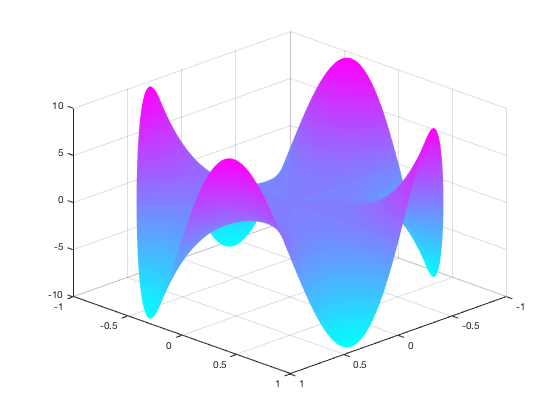
\includegraphics[width=5cm]{styles/sinBoundarysovle.png}
  \caption{$u_{sol}(x)$}%{Plot of harmonic function}
  \label{fig:swingSolve}
\end{minipage}
  \begin{minipage}[b]{0.4\textwidth}
  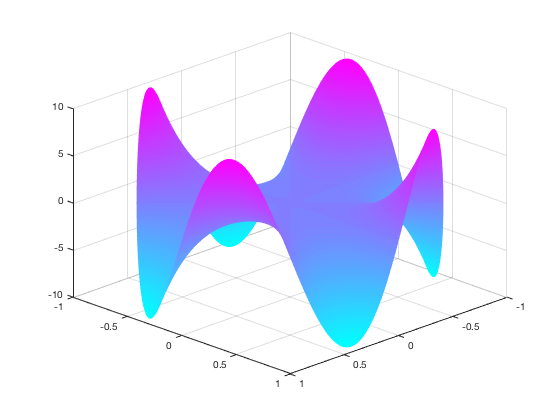
\includegraphics[width=5cm]{styles/swing_function_plot.png}
  \caption{$u(x)$}%{Numerically solved solution}
  \label{fig:swingPlot}
  \end{minipage}
\end{figure}

On the left, the numerically solved solution of harmonic \GLS{PDE} given the boundary
function $u(\phi)=10*\sin(4*\phi)$.  On the right, the solution function $u(r,\phi)=r^{4}*\sin(4*\phi)$
can be seen. Both plots are defined on the 2D unit circle $\Omega$.  Both approaches
came to the same result, but for the problem on the left, a known harmonic boundary
condition was defined, and then a solution was solved for numerically.  On the right,
the solution from the left, was analytically found by applying the Laplace operator
in polar coordinates to the generalized harmonic function $r^{\alpha}*\sin(4\phi)$,
and solving for $\alpha$.

Should one integrate over the boundary $\partial \Omega$, it follows that \begin{equation}
u(a) = \int_{S}u(a + r\zeta)d\sigma(\zeta) = \int_{0}^{2\pi} 10*\sin(4*\phi)d\phi = 0,
\label{eq:radinvar}
\end{equation}
which is the solution of $u$ at the center of the 2D unit circle,
namely a =(0,0). As one can deduce from this example, in a ball, this solution is
radius invariant.  This property is one of the main key stones of \Gls{RWoS}.
%TODO: discuss the rotational independence as can be seen by the independence of
% the solution from r==> wichtig für step size beliebigkeit.
  \subsubsection{The Maximum Principle}\label{sssec:maximum}
  % how this follows from the mean value principle
  Following from \ref{sssec:meanvalue} one can make more generalized statements of
  the maximum values of harmonic functions.
  \begin{quote}
      Let $\Omega$ be connected, and let $u$ be harmonic and real valued on $\Omega$.
      If $u$ has either a maximum or minimum in $\Omega$, then $u$ is constant.\cite{Axler1992}
  \end{quote}

  This property of harmonic functions can be nicely visualized in the solution given
  in figures \ref{fig:swingPlot} and \ref{fig:swingSolve}. Were on to select any circular
  sub-domain $\omega \subset \Omega$ of the unit circle, one would notice that the maximum value is always
  on the boundary  $\partial \omega$.  Should one claim that the maximum  value be within $\omega$
  the function $u$ would have to be "flat" and therefore constant to fulfill \ref{sssec:meanvalue}.

  \subsubsection{Weighted Mean Value Principle}%Real name is the Poisson Kernel for the Ball
  % weights can be compared to probability of hitting a certain boundary based on Brownian motion.
  Building on the mean value properties of harmonic functions, one can show that if $u$ is harmonic and,
  $\bar{B}$, then

   $$u(0) = \int_{S}u(\zeta)d\sigma(\zeta),$$
  then for any $x \in B\text{, }u(x)$ can be expressed as a weighted average of
  $u$ over $S$. Furthermore, there exists a function $P(x,\zeta)$ such that
  $$u(x)=\int_{S}P(x,\zeta)u(\zeta)d\sigma(\zeta).$$  The function can be shown
  using the symmetry properties of harmonic function on a sphere to be defined as
  \begin{equation}
    \tag{Poisson Kernel for the Ball}
    P(x,\zeta) = \frac{1 - \abs{x}^{2}}{\abs{x- \zeta}^{n}}
    \label{eq:poissonkernel}
    \cite{Axler1992}
  \end{equation}
  in an $n \in \mathbb{N}$ dimensional space.

  \subsubsection{Dirichlet Problem for the Ball}
  Building on the weighted mean value principle and the maximum principle for harmonic functions
  , one can hypothesize that given a function $f$ on $S$, that a harmonic function $u$
  exists of $B$ such that $u = f$ on $S$. Essentially saying, that given the \gls{BVP},
  on a sphere, that a harmonic function can be found as the solution.  Building on
  \ref{eq:poissonkernel}, it can be shown that
\begin{theorem}
  for continuous $f$ on  $\partial B(a,r)$,
there exists a unique continuous function on $u$ on $\bar{B}(a,r)$ with $u$ harmonic on
$B(a,r)$ such that $ u = f $ on
$\partial B(a,r)$, therefore solving the Dirichlet problem on $\bar{B}(a,r)$\cite{Axler1992}.
\end{theorem}

\section{Approach}
It has been shown, that harmonic functions exhibit many unique traits and properties
that allow one to make deductions about their solutions.  The analytical search for solutions to
the Dirichlet Problem for the Ball is possible, but one would benefit greatly if
from a solving method that avoids analytical evaluation and is easily applicable on more
general boundary geometries.  To find such a solver, one can exploit the properties
of harmonic functions discussed above.  One solver that does just that is \Gls{RWoS}.
\par
 \Glspl{RWoS} is a highly parallel solver for harmonic \Glspl{PDE}, %discribe how eliptic pds can be transformed.
and enjoy greater efficiency and practicality than more common solvers e.g.
finite differences or multi-grid when sparse solutions regions are of
interest in higher dimensions \cite{DeLaurentis}\cite{Bornemann}\cite{Yang}.  The Random Walks on Spheres Algorithm
gained it's name, due to the combination of Brownian Motion, a numerical model
of the random motions of particles, and the the mathematical connection between
harmonic functions and spheres\cite{Axler1992}, to iteratively traverse a series %Markov Chain
of spheres in random brownian motion like directions % dictated by Brownian Motion ...
in order to solve a given harmonic PDE\cite{DeLaurentis}.
Brownian Motion (see \ref{sssec:brownian}) was first %TODO: glossary Gaussian plane
proposed for this application by Shizuo Kakutani in 1944\cite{kakutani},
where it was shown to be an effective tool
in solving harmonic functions in the two dimensional Gaussian plane.  This methodology has since been
shown to be applicable to N-Dimensional harmonic PDE's \cite{DeLaurentis}.  During the 1960's
and 70's it was applied to calculate hotspots in nuclear reactors\cite{Bornemann}.
% Though the applications are great, and the individual steps are simple, it is important to
%  gain a basic and intuitive the intricacies of the Random Walking on Spheres Algorithms.
% The following passages will practically explore the theory and history behind this method,
% while also touching on the mathematical foundations on which the algorithm is based.

\subsection{Monte Carlo Methods}\label{sssec:montecarlo}
Monte Carlo Methods describe statistical algorithms that are based on the sampling a
large number of random system states and classifying the resulting set\cite{Metropolis}.
Or per Bauer consist of a ''stochastic process which produces a random variable
 whose expected value is the solution of a certain problem''\cite{bauer}.
These methods became popular in nuclear research in the 1940's when practical
experiments were limited and analytical solutions were not unknown.  Monte Carlo
Methods were found to be useful when analyzing the time independent Schrödinger
Equation\cite{Metropolis}. Muller defined
Monte Carlo Methods in 1956 as: \begin{quote}[a method which for] an unknown solution to a given physical
problems being estimated by a method which essentially depends on statistical sampling technique.
This approach requires the utilization of random variables of an appropriate
stochastic process such that samples of the process yield valid statistical results\cite{Muller}.\end{quote}
This approach is the basis of The Random Walks on Spheres, when solving harmonic \Glspl{PDE} as described in the
following passages.
%TODO pi example?
\subsection{Random Directions and Uniform Distributions on Spheres}
Given the great importance of random directions for \Gls{RWoS}, a brief excursion
into how one can numerically create a uniform distribution on a sphere can prove
to be helpful and insightful.
%proof using definitions of sin and cosine similar to the inverse of Tschebychev points
\cite{Yang,Muller1959,marsaglia1972}


% \subsection{Markov Chains}\label{sssec:markov}
% A Markov Chain is a term used to describe a series of independent events or ''states'',
% who's transition probabilities, i.e. the probability of switching from one state to the
% next, is in independent of past states.  Mathematically this process is described by Howard as:
% \begin{definition}
%   for the set $S$ defined as the finite set of $N$ states, where $s_{i}=\{s_{1},s_{2}\ldots,s_{N}\}\in S$, for simple
%   Markov Processes, the probability of transitioning from state $s_{i}$ to the following state
%   $s_{j}$ is defined by the the probability $p_{ij}$ where $\sum_{j=1}^{N} p_{ij}=1$ and $0 \leq p_{ij} \leq 1$.
%  \cite{howard}\cite{diaconis}.\end{definition}
% In the first pages of his book, Howard graphically depicts this process as,
% \begin{quote}
% ''a frog in a lily pond.  As time goes by the frog jumps from one lily pad to another
% according to his whim of the moment.  The state of the system is the number of the
% pad currently occupied by the frog; the state of the transitions is the course of his leap''
% \cite{howard}\end{quote}
% When the space $S$ is considered to be continuous time, one can speak of a Wiener Process.
%
% %TODO: convergence as in \cite{diaconis}
% \cite{Grindstead}
% \cite{howard}
%
% \subsection{Brownian Motion}\label{sssec:brownian}

\section{The Random Walks On Spheres Algorithm}
\Gls{RWoS} is a numerical Monte Carlo Method which employs Brownian Motion
like random walks to stochastically and discretely solve
harmonic \glspl{PDE}.
\par
%TODO: define terminology that will be used in this paper.

\subsection{The Algorithm}\label{sssec:algorithm} %TODO: one or we?
Now that some of the building blocks have been covered, the individual steps of
the algorithm can be discussed.  The goal of the algorithm is to approximate
the solution $u(x_{0})$ at an interior point $x_{0}$ by randomly sampling boundary
values.  To traverse the domain  to the boundary, we implement Brownian-Like motion.
In order to reduce the number of random Brownian steps needed to reach the boundary,
one exploits radius independence of $r$ as described in \ref{eq:radinvar}.  Starting
from our origin, we find the largest sphere that can fit into $\Omega$ %reference drawing
and select the radius of this sphere as our step size $r$.  We then choose a random direction $d$
that is uniform on the sphere. %reference excursion
After we step a distance $r$ in direction $d$ and arrive at $x_{1}$, we repeat the the afore mentioned process.
This process is repeated until $x_{m}$ reaches the boundary $\partial \Omega$.
It has been shown that the probability of this occurring has been shown to be 0\cite{kakutani1944}. %analogy to overlap of tangentail line on circle.
 For practicality we insist $u_{m}$ be within an $\epsilon$ boundary of $\partial \Omega$,
 therefore ensuring boundary convergence.  After the $\epsilon$ Boundary has been reached,
 one projects $u_{m}$ to $\partial \Omega$ and evaluates $f(\overline{x_{m}})$.
This algorithm is used to sample $N$ boundary evaluations, the expected value of which,
reflects an increasingly more accurate approximation of the solution $u(x_{0})$
for ever an ever greater number of trails $N$\cite{Bornemann,DeLaurentis}.  Below, the algorithms has been
described in pseudo-code.


 \begin{algorithm}[H]{$N, eps, x0$, $\Omega$}
  \caption{Walking On Spheres}
 \label{alg:wos}
\begin{algorithmic}[1]
   \State $dim \gets length(x)$ \Comment{dimension determined by size of $x0$}
   \State $ r \gets INFINITY$
  \For{$i\gets0,N$} \label{lst:line:for}
   \State $x \leftarrow x0$
   \While{$r>eps$}
      \State find largest sphere radius $r$ in $\Omega$ with center $x$ \label{lst:line:radius}
      \State find uniform random direction $d$ on sphere \label{lst:line:direction}
      \State $ x \gets x + r * d$ \Comment{update current location}
 \EndWhile
 \State $\overline x \gets project(x)$ \Comment{Project to boundary }
 \State $E \gets f(\overline x)$ \Comment {evaluate boundary value }
 \State $sum \gets sum + E$ \Comment {add result to partial sum} \label{lst:line:reduce}
  \EndFor
 \State $\textbf{return} \text{ } sum / N$ \Comment{return expected value}

\end{algorithmic}
\end{algorithm}

The intrinsic parallelism in this algorithm is plain to see, namely, one can easily
exploit the independence of each individual path by exciting all paths in parallel.
This can be realizing by unrolling the for loop in algorithm~\ref{alg:wos}, line~\ref{lst:line:for}.
The resulting values $E$ can also be reduced in parallel (algorithm~\ref{alg:wos}, line~\ref{lst:line:reduce}).  Furthermore, for every path step,
the radius and direction are independent (algorithm~\ref{alg:wos}, line~\ref{lst:line:direction} \&~\ref{lst:line:radius}),
 and can therefore be computed in parallel. \cite{Muller,DeLaurentis,Bornemann}

\section{The Basics of Parallel Computing}
In recent years, the convergence towards the physical limits of Moors law has lead to a
trend towards Parallel Computing\cite{Kumar}\cite{Markov}.  By most accounts, the
field of Parallel Computing conceived in the early 1958\cite{Gill}, but had previously
been discussed (e.g. Metropolis \cite{Metropolis}). Since then, the field has
 bloomed into the State of the Art for high-dimensional simulations and
 other highly parallel applications in
High Performance Computing as hardware technology has caught up to the first
theoretical speculation of half a century prior. \par

Traditionally, the concept of Parallel Computing was simple; in order to improve
(reduce) computation time, one should separate independent steps of a given algorithm
and execute them concurrently upon unique processing units.  In doing so, for a given
problem, which traditionally would have taken time \textit{T}, in the optimal case,
the calculation could be completed in \textit{T/N} time, where \textit{N} describes
the number of unique processing units being utilized.  This observation was formalized
by Gene Amdahl in 1967\cite{Wilt}:
%
\begin{equation}
  \tag{Amdahl's Law}
  speed-up = S_{latency}(s)= \frac{1}{(r_{s} + \frac{r_{p}}{N})} = \frac{N}{N(1-r_{p})-r_{p}}
  \label{egn:Amdahl}
\end{equation}
%
where \textit{\gls{speed-up}} embodies the factor of temporal acceleration a program
exhibits when additional computational resources are dedicated to it's execution.
The variables \textit{$r_{s}$} and \textit{$ r_{p} $} represent the percentage of
 the algorithm that must be executed serially or in parallel, respectively.
   Amdahl's Law describes a computational problem of a fixed dimension,
and the effects of more parallel computing resources on execution time.
This strategy of optimization, in which the size of the problem is constant,
 is called Strong Scaling.
In extreme cases unlimited resources, the greatest speed up of a given algorithm
 is limited by it's serial component.
%
\begin{equation}
 \lim_{N\to\infty}  \frac{1}{(r_{s} + \frac{r_{p}}{N})} = \frac{1}{r_{s}} = \frac{1}{1-r_{p}}
\end{equation}
%
This description of optimal \gls{speed-up} does not take into account issues of physical
distance of computing cores or the communication and facilitation overhead between
cores that can occur in real applications, which can lead to lower parallel efficiency.
Nevertheless, the model can serve as a benchmark when analyzing algorithmic
parallelization and  the greatest attainable speed-up for a given problem.\par

One further method of quantifying parallelism, is Gustafson's Law\cite{Gustafson}.
%
\begin{equation}
  \tag{Gustofson's Law}
  speed-up = S_{latency}(s) = r_{s} + (1 - r_{p})N
\end{equation}
%
This view of parallelism maintains that `` in practice, the problem
size scales with the number of processes'', and therefore
``assume[s] run time, not problem size, is constant''.
of the given problem. In other words, as the problem size grows, a proportional
amount of resources should be devoted to keep the execution time constant.
Both of these laws, assist in the quantification of parallel efficiency and
expected gains.

\subsection{GPU Hardware}
When looking to implement efficient numerical code, it is important to understand
 the underlying hardware, in order to exploit architectural intricacies for performance gains.
 To this end, the following passages will be a deep dive into into the History of
 computer architecture and subsequently the design of NVIDA \Glspl{GPU}.
\par
Modern computing architecture was first proposed by John Von Neumann in 1945\cite{vonNeumann}.
This architecture is composed of three separate sections: the \Gls{CPU}, memory, and \Gls{I/O}.
Modern \Glspl{CPU} are comprised of an \Gls{ALU} comprised of electrical circuits
perform basic mathematical operations, such as addition, subtraction, multiplication and division,
registers, which store the data used for computation by the ALU and Cache, which is a more modern development to improve data locality.
\par
By design, \Glspl{CPU} are constructed
to handle general purpose computing workloads.
An \Gls{ALU} computational
tasks on an individual datum. By the nature of this
generalized strategy, upcoming computation steps and which data are therefore required,
is unknown to the \Gls{ALU}. If the ALU does not have the data necessary for a computation,
it is forced to wait for the data to be fetched from memory, which can greatly increase computation time.
\par
Transfer times from \Gls{RAM}
are orders of magnitude greater than the computation clock frequency of
a CPU.  This is due to the relatively large physical separation between the CPU and memory,
 the communication overhead needed to fetch the data, and
the nature of \Gls{DRAM}, which electrically refreshes data values at a designated rate.
These problems together are referred to the Von Neumann Bottleneck\cite{Backus}.
It is important therefore, to develop algorithms and strategies that  predict which data will be required by upcoming operations.
A main focus of modern CPU computation strategies, is to always ensure that the data
necessary for a computation is at hand, ready to be used, when requested by the \Gls{ALU}.
The limited number or registers on the ALU meant anohter, more local storage mechanism
was required.
\par
Cache is a bank of \Gls{SRAM}
that is etched on the same silicon wafer as the CPU itself.  This physical locality,
along with the higher read and write speeds compared to \Gls{DRAM}, lessen the transfer
time of data to the registers, and therefore increase the effective ability of the
 \Gls{ALU} to complete computations.
Due to the greater production cost of on-chip Cache, its size is limited, and
much research has been dedicated to optimizing cache load strategies of modern CPUs. %TODO cite
\par

It is important to grasp the strengths and weaknesses of modern \Glspl{CPU} to
recognize the computational benefits of \Glspl{GPU}
for modern computations problems.  As the name eludes, \Glspl{GPU} were originally developed
as dedicated computational units for 3D graphics\cite{Sanders}.  They are housed on the same
communication bus as the \Gls{CPU} and memory, and assigned image computational work,
to lessen the load of the \Gls{CPU}.
The GPU specifically designed to handle workloads on large data sets (traditionally these
data sets were individual color values for digital images, and the workload as
the transformation of image data to modulate the output on a digital screen).
This heritage,
defined the strategy modern GPUs take towards computation.
The image data was was relatively high dimensional with intensity values for every pixel in the image.
Each pixel was at least three dimensional (one dimension per color value of red, green and or blue) and
some had a fourth value for alpha transparency. These values would often all undergo
well defined modulation, that could be formulated in a function based on position values.
In the early 2000's these functions were named shaders, and later kernel functions.\cite{5751939}
Due to the independent nature of the execution of kernel functions, the GPUs have multiple, less robust
arithmetic units, that perform an individual instruction set on more well defined data.
The well defined execution order leads to less overhead in the execution
model, allowing more resources to be devoted to computation.
Due to the dimensionality of the data being computed, \Glspl{GPU} have larger registers\cite{5751939},
which allow for fewer context switches, and therefore greater \gls{ai}.  Overall
Through put is valued more than single thread execution speed.  %lower thermal density?

%TODO: expand
\subsection{GPU Architecture}\label{ssec:gpu_architecture}
The GPU hardware architecture and terminology of said architecture varies from
vendor to vendor.  For the sake of uniformity, this document will adopt the
terminology employed by the manufacturer, NVIDIA.  To begin, in the following passages the CPU
will be referred to as the \textbf{host} while the GPU will be called \textbf{device}.
These are standard terminologies in GPU programing. GPUs are comprised of four major components:
\begin{description}
  \item[Host interface] moderates communications between the host and the device.
  Commands are dispatched to the necessary hardware, and synchronization between
  host and device is managed through this interface.
  \item[Copy Engine] manages the bidirectional transfer of data between the host
  and device.  Modern hardware can have 0-2 Copy Engines per device in order to
  manage the conversion of linear memory to CUDA arrays while saturating the PCI
  bus.  The independence of the Copy Engine(s) allows for concurrent data transfers
  and computation.
  \item[DRAM Interface] a memory interface with a bandwidth of up to 100Gb/sec\cite{Wilt}.
  Some interfaces also support device side L2 caches usage.
  \item[TCPs \& GPCs] \underline{T}exture \underline{P}rocessing \underline{C}luster
  and \underline{G}raphics \underline{P}rocessing \underline{C}lusters are an assembly
  of \Glspl{SM} along with cache for computation.
\end{description}\cite{Wilt}

\subsubsection{Streaming Multiprocessors}
Each GPC contains a cluster of SM's.  The number of SM's per cluster varies by
model of GPU. Some examples can be found in %table bellow

%TODO list table with modern examples

Each SM is comprised of: \cite{Wilt}
\begin{itemize}
  \item execution units for 32-bit integer, as well as single and double precision arithmetic.
  \item Special function units for log/exp sin/cos and sqrt functions.
  \item a warp scheduler to coordinate the dispatch of threads.
  \item a constant cache to broadcast data to SM's.
  \item shared memory accessible by all threads.
  \item texture mapping hardware.
\end{itemize}

This basic overview of the architecture of the hardware is important to understand
how the the programming API maps to the available hardware.

%TODO: discuss streaming processing.

\section{Parallel Computing with CUDA}
\subsection{CUDA Software}

The CUDA parallel computing environment is a C++ language wrapper with built in
pragmas to interact with the NVIDIA hardware.  Although CUDA is modeled on the
hardware it runs on, it is not wholly analogous with the hardware architecture,
and higher level concepts have been added to aid in the implementation of CUDA code.
%TODO insert diagram of CUDA stack.
\par
The CUDA ecosystem stack is comprised of five layers accessible to the user.
These layers are the CUDA application itself, CUDA Libraries, CURA Runtime otherwise
known as CUDART, and the CUDA Driver.


\subsubsection{CUDA Libraries}

The highest level of this stack is occupied
of CUDA libraries. When looking to optimize code with CUDA, a
first step should be the implementation by CUDA Libraries.  These highly optimized
and user friendly libraries, such as CUBLAS and CUDA Thrust, allow the use of
CUDA hardware, with minimal understanding of the hardware or execution strategy.  These can prove
to be indispensable tools for beginner users or those looking to quickly and
efficiently prototype a problem. The author recommends their use as the first step
in any CUDA based undertaking. They provide the ability to create a quick proof
of concept for a project, as well as a highly optimized base line, should further
development be planned.
\subsubsection{CUDA Runtime}

Moving down the Stack, CUDA runtime provides an interface to the user, which mirrors
standard C++ functionality such as malloc and memcpy.  These functions differentiate
themselves from host functions with the preface \textit{``cuda''} or \textit{``cu''}
e.g. cudaMalloc and cudaMemcpy.  Functions that are to be excited on the
device, are called kernels or kernel functions, which can be identified
 via their triple angle bracket syntax, ``$<<< >>>$''.
%TODO example of basic CUDA kernel
Kernel parameters can be specified in these triple angle brackets.  These parameters
include number of blocks per grid, threads per blocks, size of shared memory and
stream, all topics witch shall be discussed later in this document. %TODO cite where.

%TODO describe blocks and threads
\subsubsection{CUDA Driver API}
The CUDA driver is the interface to lower lever command sets used by the CUDA driver, which allows more detailed control
of kernel calls and memory allocation. Many of the same functionalities are possible,
but execution is more tedious and requires steps \cite{driver}. This granularity of control can nevertheless be
helpful when tuning a program and striving for higher execution performance.
\subsubsection{CUDA Driver}

The CUDA driver is the lowest level of integration between the host and the device
and facilitates communication between the \Gls{GPU} and the rest of the computer via the bus. %TODO: define Bus.


\subsection{Compilation and Execution}

%TODO: Make diagram. CUDA book page 58

CUDA programs are written in CUDA flavor C++.  The CUDA wrapper of C++ is the
compiler driver nvcc, which can compile, link and execute CUDA code.  This process occurs
 in three main steps.
 \begin{enumerate}

\item First,
files containing CUDA pragmas are assigned the .cu ending format, and split upon
compilation into device and host sections.
\item Second, these files are subsequently
compiled separately into to host and device machine code respectively.
\item Lastly, both compilates are merged into a single executable, to be run on the host.
\end{enumerate}
\par
Device machine code, is referred to as \hyphenation{mi-cro-code} \textit{microcode},
which is compiled for a specific device model's architecture. In order to be able
to execute the same executable
on multiple \Glspl{GPU} and to allow backwards compatibility of CUDA features, CUDA code is
first compiled into \Gls{PTX}, a pseudo-assembly language.  \Gls{PTX} is then
further compiled in to device microcode and written into a CUDA binary file called .cubin.
This can either happen offline, at compile time,
or online, at runtime, in a \gls{jit} fashion.  By default, both
the microcode for the local device present at compilation and the generalized
\gls{PTX} compilates are added to the to the executable file.
This way, should the executable be run on a different device, the \gls{PTX} can
be recompiled appropriately with \Gls{jit} compilation, and executed on the a
desired device\cite{Wilt}.

\subsection{Programming CUDA}

There are many parallel contexts when programming CUDA. To help developers conquer
the challenges of parallel programming, CUDA offers a multi-contexts development
environment to help break problems down into sub-problems, that can be then translated
by the compiler into parallel code. The following explanation, is only meant to
give the reader insight into the CUDA syntax, thereby allowing comprehension of
the following work. For a more complete and elaborate explanation of CUDA, other
more extensive resources are recommended\cite[e.g.]{Wilt,Sanders,driver}.
%separate address space from CPU --> mem copies
%blocks and threads
\subsubsection{Blocks, Threads and Grids}
%TODO: insert diagram of threads blocks and grids
The two main contexts of parallelism in CUDA are CUDA blocks and CUDA threads.
Threads can be thought of as individual registers, with an assortment of computational
functionality.  Threads should be considered to be completely independent from one another,
and only synchronized through explicit call to synchronization functions. Threads, like
registers, can only work on one datum at a time, but are all executed simultaneously.
Threads are, in turn, organized into blocks, and a collection of blocks comprises a grid.
Blocks could be explained as a process on an SM. If resources allow, multiple blocks can
be executed on an \Gls{SM} simultaneously. Since neither the number of blocks nor the
number of threads are limited by the limited by the number of registers and \Glspl{SM},
but rather can exceed hardware values, the analogy stops here.  Both
threads and blocks can be described by an abstraction of a hardware feature, although one should try to
consider hardware and software separately from one another, as to reduce the number
of false assumptions.
\par
For ease of programming, the current thread or block ID can be retrieved using
 threadIdx.\{x,y,z\} and BlockIdx.\{x,y,z\}. As can be deduced via the nomenclature,
 these variables are multi-dimensional, a feature that can be advantageous in some
 applications such as computer vision, but is not a necessity in other applications
where the problem does not map to a 2 or 3D euclidian space. Further variables,
for the dimension of the grid and block are also available. %TODO: Create table as on page 213
The number of threads and blocks assigned to a problem is relatively arbitrary and can
be designated by the developer before hand, or dynamically.  There are however limits
to this flexibly that are described in the CUDA documentation\cite{bestpractices}.
  Also, minor performance
repercussions could be experienced, if the dimensionality of the framework is poorly
chosen.
%TODO: stream processing?
%kernel syntax
\subsubsection{Kernels}

At the core of any CUDA program, is the kernel. Kernels make up the basic instruction
set what one often finds in any other serial program as well, the only difference being,
where as in a serial program one would iterate over data by means of a loop,
CUDA kernels are executed on every data in an array.

%TODO: vector addition example

The angle brackets in front of the kernel call, identify the function as a kernel,
and allow syntax  identification during compilation of a program.  Depending on
whether a device kernel is to be called from the host, or internally from the device,
kernels can be labeled with the pragma \_\_global\_\_ or \_\_device\_\_  respectively.
Kernels declared \_\_global\_\_ can be called from both the host and device, while \_\_device\_\_
kernels are only available from the device. %TODO: why is this the case? why is this important?
The identifier \_\_host\_\_ allow for kernels to be called from and run on the host.

The parameters in the triple angle brackets are in order, grid size or number of blocks,
block size or number of threads, size of shared memory, and stream ID.  While grid and block size,
are required values, the size of shared memory can also be statically allocated from within
a kernel (more on shared memory in \ref{sssec:memories}).  Dynamic allocation though requires the kernel to be called parameterized with
the size, and the value to be initialization from within the kernel function.  The stream
parameter also is set to main stream by default, but must be set by the user when
working with multiple streams (more on streams in: \ref{sssec:streams}).
%shared vs. global memory
\subsubsection{Memories}\label{sssec:memories}
GPU memory does not benefit from features such as virtual
memory or paging, as one might expect from CPU memory. Instead devices have an
address space completely separate from the host address space, where every address is assigned a physical space in memory.
In many cases memory consists of a dedicated chip on the device that is controlled
by the memory controller.  This memory must be managed by the user when programming in CUDA.
\par
Not all device memories are created equal.  Similarly to \Glspl{CPU},
different memories have varying strengths and weaknesses.  By preallocating memory for a variable,
that is either read only, or read and written often, one can greatly increase the
performance of ones program\cite{Wilt}.   %TODO: CUDA attempts to avoid lazy allocation--> performance gains.
There are four main types of CUDA memories.
\begin{description}
  \item [Global memory] Memory on the Device with bandwidth of up to 100 Gb/sec.
  Global memory is allocated dynamically by the user via cudaMalloc() and cudaFree() functions.
  Dynamic allocation is normally performed in host code, due to large performance short fall
  when implemented in a kernel call.
  %TODO: coalescing?
  \item [Constant memory] optimizes for read only memory on device for higher
  read speeds.  The constant declaration is beneficial for broadcast style data
  reads, in other words, when every thread is to receive the same data.
  \item [Texture memory] Constant declaration of global memory with dedicated
   texture access pattern controller.  Texture memory allows performance benefits
   for uncoelessed variable access, which would normal lead to large performance
   degradation with normal global memory.
  \item [Shared memory] User managed cache located on every \Gls{SM}.  Shared memory access
  normally benefits from a 10x speed increase over global memory access, while it remains
  10x slower than register reads.\cite{Wilt} %TODO: shared memory coalescing.
  \item [Local memory] local memory contains the program stack for every thread
  in a CUDA program. Should a program run out of registers for thread local variables,
  local memory is  used to store overflow variables. This variable overflow is often
  linked to detrimental performance losses and should be avoided.\cite{Wilt}
  \item [cache]
  \item [registers] Memory units on \Gls{SM} used to store thread local variables,
                    and variables for current computation.
\end{description}

%streams
\subsubsection{Streams}\label{sssec:streams}
CUDA Streams enable the coarsest level of concurrency in the CUDA API.  Streams
are consist of a series of commands that are to run in series.  Commands assigned
a different set of streams can be executed in parallel. Memory transfers and
kernels can be separate stream in order to create a workflow pipeline and increase
the overlap between data copying and data modulation. This is made possible by the
independent Copy engine as mentioned in \ref{ssec:gpu_architecture}.  Furthermore,
on systems with more than one \Gls{GPU}, streams can allow both data transfers and
kernels to be excited concurrently on separate \Glspl{GPU}, leading to even greater
performance.




	 % ---------------------------------------------------------------------------
	 %
	 %
	 %
	 % ---------------------------------------------------------------------------
	 \part[Implementation and Experiments]{Implementation and Approach}
   \chapter{Approach}
\label{chapter:approach}

\section{Experiment Hardware}
For the numerical experiments conducted during this research, two hardware configurations
are used.  First, a dual GPU configuration consisting of two NVIDIA GTX 560Ti GPU's is
employed to test multi-device capabilities. Also, seeing as these devices
could only run \Gls{CUDA} code complied for compute architecture 2.1, code
backwards compatibility was also tested with this set up.
The second compute configuration consists of an NVIDIA TITAN X GPU, which allowed
the testing of the compute architecture 6.1.
\par
Both \Gls{GPU} configurations were run used with the same Fujitsu D3067-A1 mother board,
with 16GB or RAM and an Intel Xeon CPU, model E31235 running at 3.20GHz.

\section{Parallelization}
In order to successfully map a mathematical problem to specific hardware, one must
consider the three main bottle necks of parallel computing, namely,
memory allocation and access strategies, execution order and data communication.
The complete implementation, can be found and referenced in appendix \ref{appendix}.
In the following passages, some of the intricacies of the implementation will be
elaborated.

\subsection{Thread-level Parallelism}\label{tlp}
Commonly, one wishes to store heavily used data in shared memory in oder to
take advantage of the increased data access speeds and inter-block data sharing
capabilities.  For this reason, the \textit{direction}, \textit{radius}, and \textit{position}
vectors were all stored allocated in shared memory, contributing a shared memory usage of
$3N$.
\begin{lstlisting}[caption="src/wos\_native.cuh",label=BlockVariablePointers]

  struct BlockVariablePointers {
    float *s_radius, *s_direction, *s_cache, *s_x, *s_result;
  };
  __device__ void calcSubPointers(BlockVariablePointers *bvp, size_t len,
                                  float *buff) {
    bvp->s_radius = buff;
    bvp->s_direction = len + buff;
    bvp->s_cache = 2 * len + buff;
    bvp->s_x = 3 * len + buff;
    bvp->s_result = 4 * len + buff;
  }
  __device__ void smemInit(BlockVariablePointers bvp, float *d_x0, int tid) {
    // initialize shared memory
    bvp.s_direction[tid] = 0.0;
    bvp.s_cache[tid] = 0.0;
    bvp.s_radius[tid] = INFINITY;
    // copy x0 to local __shared__"moveable" x
    bvp.s_x[tid] = d_x0[tid];
    if (threadIdx.x == 0)
      bvp.s_result[0] = 0.0;
  }
\end{lstlisting}

For each dimensional vector entry, one thread was assigned, subsequently
also leading to a \textit{blocksize} of $N$.  The practice of one tread per vector
entry is a common pattern in many \Gls{GPGPU} as is the pattern of storing data in shared
memory and using one thread per data entry enables efficient data communication
between threads and accelerated data reads from shared memory. In order to allocate,
and initialize and manage multiple variables in shared memory, a pointer structure and helper functions
were used.  This structure was initialized locally per thread and pointed to an
external allocation of shared memory $buff[ ]$.

Each of the steps of \Gls{RWoS} was implemented thread-wise.  A thread-wise implementation
explicitly defines a each step as a kernel for individual vector entries.  Each of these operations
can be executed in parallel by its respective thread.  Where communication is necessary,
shared memory access and a function call $\_\_syncthreads()$ in order to avoid \Gls{rc}.

\subsection{Block-level Parallelism}
Due to the lack of communication necessary between independent paths and their
their subsequent boundary evaluations, the mapping to \Gls{CUDA} blocks lends itself
to the  application.  For the evaluation of $P$ \Gls{RWoS} paths, $P$ CUDA blocks
of dimension $N$ are allocated.  Each local Path evaluation result is saved in the $s\_result$
variable in the shared memory structure \ref{BlockVariablePointers}.
\par
In mapping every path to a specific block, one limits oneself to the bounds of the
CUDA hardware.  Currently, the greatest number of blocks available for execution
of one kernel limited to the value $MAX\_BLOCKS = 65535$.  In oder to reach a greater
iteration count, a strategy was devised to split a number of total paths greater
than $MAX\_BLOCKS$ on to a smaller number of \Gls{CUDA} resources.  This strategy,
although primitive, was found through testing to yield the greatest performance,
compared to all other tested strategies. One can assume, this is due to greater
explicit dependency independence that the a block exhibits.  All other alternatives,
involved a greater number of "sequential" path evaluations per block, and therefore
a greater overall running time.   Meanwhile, by maximizing the number of blocks,
one creates greater parallelism in the program that can be exploited on a \Gls{GPGPU}.
An excerpt of the implementation can be found below.

\begin{lstlisting}[caption="src/gpu\_config.cpp Appendix \ref{appendix}",label=block-parallelism-strategy]
  ...
  // uppdate paths per block
  if (gpuPaths <= MAX_BLOCKS) {
    numberBlocks = gpuPaths;
    blockIterations = 1;
    blockRemainder = numberBlocks;
  } else {
    numberBlocks = MAX_BLOCKS;
    blockIterations = ceil((gpuPaths / (float)MAX_BLOCKS));
    blockRemainder = gpuPaths % MAX_BLOCKS;
  }
...
\end{lstlisting}

\subsection{Device-level Parallelism}
In order to decrease running time, it is advantageous to map the problem at hand
to multiple devices.  In the course of this work, this was realized through a
simple stream based distribution to two devices connected by a common PCIe bus.
The strategy for device level parallelism was precedes the block-level parallelism
strategy, and merely divides the total number of paths desired, by the number of
available devices.
\begin{lstlisting}[caption="src/gpu\_config.cpp Appendix \ref{appendix}",label=device-parallelism-strategy1]
  //...
// nGPU
checkCudaErrors(cudaGetDeviceCount(&nGPU));
gpuPaths = p.totalPaths / nGPU;
  //...
\end{lstlisting}

\begin{lstlisting}[caption="src/wos\_native.cuh Appendix \ref{appendix}",label=device-parallelism-strategy2]
  for (int i = 0; i < gpu.nGPU; i++) {
    checkCudaErrors(cudaSetDevice(i));
    checkCudaErrors(cudaStreamCreate(&multiGPU[i].stream));
    //...
    }
  //...
  for (int i = 0; i < gpu.nGPU; i++) {
    checkCudaErrors(cudaSetDevice(i));

    dim3 dimBlock(gpu.numThreads, 1, 1);
    dim3 dimGrid(gpu.numberBlocks, 1, 1);

    cudaError err;

    WoS<<<dimGrid, dimBlock, gpu.size_SharedMemory, multiGPU[i].stream>>>(
        multiGPU[i].d_x0, multiGPU[i].d_paths, multiGPU[i].d_avgPath,
        multiGPU[i].d_stepCount, p.eps, p.x0.dimension, p.avgPath,
        gpu.blockIterations, gpu.blockRemainder, i + 1);
    err = cudaGetLastError();
    if (cudaSuccess != err) {
      printf("Wos Kernel returned an error on device %d:\n %s\n", i,
             cudaGetErrorString(err));
    }
  }
  //...
\end{lstlisting}



\subsection{Reduction}
Data reduction describes the act of consolidating a large amount of values to
a individual value or subset of values by means of a numerical or logical operations.
Although summation is a common example, other reduce operations include,
but are not limited to maximum value, minimum value, product and bitwise reduce operations.
  Commonly,
sum-reduce describes the addition of all data values in a set and returning a single value.
In sequential execution, a reduce operation will, for $N$ input values, have a nominal
running time of $0(N)$ and is most commonly realized by means of a loop over that
input data.  In parallel computing, these operations are performed in parallel by dividing the,
workload among the $w$ worker cores and performing serial reduction of the subsets,
while finally reducing the intermediate results.  This naive approach leads to an
optimal \gls{speed-up} of $w$.  Due to the lack of a global synchronization mechanism
on \Glspl{GPU}, this naive reduction parallelization approach is not possible,
and other methods have been developed.  Mark Harris, dives deep into the benefits
and pitfalls of parallel reduction on \Glspl{GPU} and has derived optimized
recursive approaches, as documented in \cite{harris}.  Some key points from his work are
the avoidance of:
\begin{description}
  \item [Avoidance of branch divergence]
since each warp executes one common instruction at a time, when branch divergence,
(i.e. if/else evaluation) occurs for individual elements, the warp-wise execution pattern
is broken, and additional warps must be executed for diverging threads. This \Gls{GPU} anti-pattern
leads to execution overhead and a subsequent loss in performance
  \item [Bank conflict free addressing strategies]
  in order to achieve the improved performance and concurrent read and write capabilities
  of shared memory, memory is divided into equally sized sub modules, called banks.
  These sub modules can be accessed by independent threads in parallel, allowing a speed up
  of $B$ for $B$ separate memory banks.  When multiple threads request access to
  the same memory bank, the accesses are serialized, therefore restricting the performance increase.
  These access patterns are called bank conflicts, and can drastically decrease
  the performance of shared memory.  To avoid bank conflicts, a coalesced data
  access pattern is recommended.
  \item [Loop unrolling] by explicitly defining looped operations, the loop overhead
  can be reduced to a minimum, therefore allowing for greater performance during execution.
  \item [compile time evaluation]  In order to reduce the number of conditional
  evaluated at runtime, the C++ feature of templating can allow compile-time statement
  evaluation, for example concerning block and thread dimensional conditional statements.
  This pattern further increases code performance on \Glspl{GPU}
\end{description}

  \begin{lstlisting}[caption="src/wos\_native.cuh",label=sumReduce]
    //...
    __device__ void warpSumReduce(float *sdata, int tid) {
      // each thread puts its local sum value into warp variable
      float mySum = sdata[tid];
      unsigned int blockSize = blockDim.x;

      // do reduction in shared mem

      if ((blockSize == 1024) && (tid < 512)) {
        sdata[tid] = mySum = mySum + sdata[tid + 512];
      }

      __syncthreads();

      if ((blockSize >= 512) && (tid < 256)) {
        sdata[tid] = mySum = mySum + sdata[tid + 256];
      }

      __syncthreads();

      if ((blockSize >= 256) && (tid < 128)) {
        sdata[tid] = mySum = mySum + sdata[tid + 128];
      }

      __syncthreads();

      if ((blockSize >= 128) && (tid < 64)) {
        sdata[tid] = mySum = mySum + sdata[tid + 64];
      }

      __syncthreads();

    #if (__CUDA_ARCH__ >= 300)
      if (tid < 32) {
        // Fetch final intermediate sum from 2nd warp
        if (blockSize >= 64)
          mySum += sdata[tid + 32];
        // Reduce final warp using shuffle
        for (int offset = warpSize / 2; offset > 0; offset /= 2) {
          mySum += __shfl_down(mySum, offset);
        }
      }
    #else
      // fully unroll reduction within a single warp
      if ((blockSize >= 64) && (tid < 32)) {
        sdata[tid] = mySum = mySum + sdata[tid + 32];
      }

      __syncthreads();

      if ((blockSize >= 32) && (tid < 16)) {
        sdata[tid] = mySum = mySum + sdata[tid + 16];
      }

      __syncthreads();

      if ((blockSize >= 16) && (tid < 8)) {
        sdata[tid] = mySum = mySum + sdata[tid + 8];
      }

      __syncthreads();

      if ((blockSize >= 8) && (tid < 4)) {
        sdata[tid] = mySum = mySum + sdata[tid + 4];
      }

      __syncthreads();

      if ((blockSize >= 4) && (tid < 2)) {
        sdata[tid] = mySum = mySum + sdata[tid + 2];
      }

      __syncthreads();

      if ((blockSize >= 2) && (tid < 1)) {
        sdata[tid] = mySum = mySum + sdata[tid + 1];
      }

      __syncthreads();
    #endif

      if (tid == 0)
        sdata[0] = mySum;

      __syncthreads();
    }
    //...
\end{lstlisting}
Briefly, the $\_\_\_shfl\_down(...)$ command should be examined. Before, compute capability
3.0 (Kepler), reductions between warps of the same thread had to be completed in
shared memory.  This meant that data transfers between warp registers and shared
memory had to be completed for every reduction step.  Since Kepler, warps have gained
the capability to directly access values stored in neighboring warps registers,
thereby increasing effective bandwidth, freeing shared memory and eliminating the
necessity for warp synchronization. This action was cleverly named shuffle \cite{shuffle}.
\subsubsection{Local Reduction}
Based on \cite{harris}, optimized reduction kernels were introduced for efficient
shared memory minimum and summation reductions needed for \Gls{RWoS}\ref{appendix}.
In order to successfully use these optimized reduction techniques, the memory allocations
discussed in \ref{tlp} were step-wise over allocated, meaning it was ensured that
the total size of allocated shared memory could store a power of 2 number of elements,
regardless of the required dimension.  Unused elements were initialized with with
values which would remain constant during the entire simulation (e.g. 0 and INFINITY).
This strategy allowed for coalesced warp-wise memory accesses, that minimized
thread divergence and despited the computational overhead, lead to performance gains
of $~50\%$ compared to initial naive reduction implementations.
\subsubsection{Global Reduction}
The global reduction of path evaluation results is realized through a serial
a $cudaMemcpyAsync(...)$ to the host, and a serial host reduction.  This strategy
proved to provide greater performance than a restructuring of the CUDA thread/Block
allocation and subsequent GPU reduction, due to the minimization of GPU configuration
overhead.  In order to reduce the numerical error of floating point reduction,
Kahan's summation algorithm was employed.
\begin{lstlisting}
  float reduceCPU(float *data, int size) {
    float sum = data[0];
    float c = 0.f; // numerical summation error variable

    for (int i = 1; i < size; i++) {
      float y = data[i] - c; // subtract previous error
      float t = sum + y; // add corrected value to intermediate sum
      c = (t - sum) - y; // recalculate error
      sum = t; // set new intermediate sum
    }
    return sum;
  }
\end{lstlisting}

\section{Random Number Generation}
In order to generate pseudo random numbers for the random directions necessary
for \Gls{RWoS}, the \Gls{CUDA} library \Gls{CURAND} was utilized.
\subsection{CURAND}
The \Gls{CURAND} library provides an API necessary for generating high quality
pseudo random numbers.  The default pseudo random number generator XORWOW was
was used during this work\cite{xorwow}.  The CURAND implementation of XORWOW provides
a seed dependent, reproducible series of random numbers, that has
a period greater than $2^{190}$. By modulating the seed, the user is guaranteed a
different starting state and subsequent different series of pseudo-random numbers.
The device API of \Gls{CURAND} allowed
the generation of pseudo random numbers during the execution of \Gls{RWoS} and
therefore greatly reduce the amount of data transfer to the device, and therefore
the overall running time of the program.  Furthermore, the pseudo-random normal
distribution functionality of \Gls{CURAND} was used to generate normal distributions
in an $N$-dimensional euclidean space, which subsequently created a uniform spherical
distribution.
%\subsection{Pseudo-Random and Quasi-Random}
\subsubsection{Seed Independence}
In order to generate independent pseudo-random directions in every dimension,
a thread independent seed was selected, seen below.
\begin{lstlisting}[caption="Random Number Generation(source:src/wos\_native.cuh see: appendix \ref{appendix})",
  label=Random Number Generation]
  int index = threadIdx.x + blockDim.x * blockIdx.x;
  int tid = threadIdx.x;

  curandState s;
  // seed for random number generation
  unsigned int seed = index * gpu;
  curand\_init(seed, 0, 0, &s);
\end{lstlisting}
By using the global thread index as a seed, one can strive to achieve independent
sequences of pseudo-random numbers in every direction, for every path.  In order,
to guarantee the randomness caries over when using a multi-GPU hardware configuration,
the GPU-ID (starting from 1) is multiplied with the the thread index seed in order
to ensure seed independence throughout the simulation.

\subsection{Excursion: uniform random directions on a Sphere}\label{uniformPoints}

In the process of understanding how the generation of uniform distributions on
spherical surfaces can be created, the following 2 dimensional practical exemplary
experiments were performed.

In order to attain a distribution on a sphere, the process followed in this work,
consisted of creating an $N$-dimensional normal distribution in euclidian space and
sampling from the afore mentioned distribution.  The $N$-dimensional sample vector
is subsequently normalized onto the $N$-dimensional unit sphere.  Below, the process
exemplarily visualized for a 2D example.  Furthermore, the 2D case of a uniform
euclidian distribution being normalized is also exemplified, in order to intuitively
show the distributional discrepancies and obvious ill suited nature for the problem
at hand.  The two point clouds below are 2D normal and uniform distributions
respectively.  The peaks on the uniform distribution histogram stem from the corners
of the distribution in a 2 dimensional euclidian distribution.  When projected onto
the sphere, the accumulation of points in the corner of the euclidian domain create
''hot spots'' in the spherical distribution.  The two dimensional normal
distribution point cloud on the other hand, mitigates this problem due to the summation
of the tails of the distributions in the 1D plane, leading to a low probability
in the corners of the square domain.  When the point cloud  is subsequently projected
onto the sphere, it lacks the peaks in the  spherical distribution and displays an
overall uniform nature as can be seen in the relatively constant levels  histogram below.


%The connection between normal distributions and spheres is not merely

%http://math.stackexchange.com/questions/28558/what-do-pi-and-e-stand-for-in-the-normal-distribution-formula

	 \label{part:secondP}

	 % ---------------------------------------------------------------------------
	 %
	 %
	 %
	 % ---------------------------------------------------------------------------
	 \part[Implementation and Experiments]{Implementation and Approach}
   \chapter{Experiments and Evaluations}
\label{chapter:experiments_and_evaluations}
For the following tests, the second computational configuration of one NVIDIA TITAN X GPU
was used.  Only for the multiple device execution section was the first configuration implemented.
\section{Software Usage}
Besides the NVIDIA CUDA ecosystem, peripheral tools are offered to allow developers
to analyze program performance, and automatically recommend tips to increase performance.
Two such programs are \textit{nvprof}, a profiling tool comparable to gprof, and
\textit{nvvp}, a visual profiler for \Gls{CUDA} software. Both tools allow developers
to discover hot spots in their programs, optimize occupancy, the amount of registers
in use on an SM, and improve data transfer strategies.  For \Gls{RWoS}, occupancy
and computational intensity were both points of great interest. Since \Gls{RWoS}
is computer bound, rather than memory bound, the goal of this work was to continually
analyze and improve compute performance.  Data transfer optimization becomes of interest
when the dimensions and number of paths become so large, that intermediate results,
can no longer be stored on the device.  In this case a stream pipeline of concurrent
data transfer of intermediate results to the host, and computation would be of great
importance.  For this proof of concept implementation, the number of paths, and dimensions
are still low enough that pipelining was not yet necessary.  Nevertheless, \textit{nvvp}
was used to analyze the computational intensity of \Gls{RWoS} for \Glspl{GPU}.
\section{Profiling}
When profiling the code, it became apparent that since the code scales with the problem
size, i.e. dimension and number of path iterations, so to does the efficiency.  Occupancy,
describes the percentage of the number of CUDA cores on an individual SM filled
by the execution of a kernel.  This
percentage is therefore dependent on the number of CUDA cores available in the hardware at hand,
and the allocated number of threads per Block.
Due to the tread allocation strategy described in \ref{localRed}, occupancy was $50\%$
for dimensions bellow 32 and $93.9\%$ for dimension=64 due to the 64 CUDA cores
per SM in the TITAN X (see: \ref{hardwareTable}). For thread allocations greater than
64, occupancy remains at around $100\%$ threads are processed warp-wise, and 2 warps can
fit on one SM. Due to the near constant computational dead-time required for memory transfer time,
greater computational intensity can be achieved with higher dimensions or path iteration values.
\par
When profiling with \textit{nvvp} it was also reviled that the current implementation,
profiled with $dimension=64, iterations=10^{6}$, displayed a relatively low warp
execution efficiency of $56.2\%$.  This was due to a large number of predicated
instructions necessary to the computation.  According to \textit{nvvp}, if one
neglects the predicated instructions, the execution efficiency would be $100\%$.
Improving the warp efficiency would be a great starting point for future work.

\section{Execution on Multiple Devices}
To increase the performance of \Gls{RWoS} for \Glspl{GPU}, a multi-device implementation
was tested.  The goal was to gain a speed-up of 2 when running the code on two devices
simultaneously.  In order to divide the workload to two devices, the total number
of path iterations desired was divided by the number of devices available. Since
result precision depends on the order of the number of iterations, is not dependent
on the exact number of iterations, the the total divided using integer devision,
and rounded to the nearest natural number for the sake of simplicity.  The two
devices selected were GTX 560Ti. As mentioned in \ref{devicePar}, the code
was run simultaneously on both devices via CUDA streams, and the results were reduced
on the host, as before. To to space constrained on the motherboard, a PCIe-extender
ribbon cable was used to conned the second device to the motherboard. Initial tests
showed that for our test case (Dimension=512, Paths=65335) the running time dropped from
30.7 seconds for a single device, to 17,9 seconds when running on two devices,
resulting in a speed up of: $$ speedup = \frac{31.7 sec}{17.2 sec} = 1.84.$$ Unfortunately,
due to hardware failure (the PCIe extender cable was not very robust), further testing
of multiple device execution was not possible.  Nevertheless, the resulting code
is able to run on multiple devices, and will automatically run on all devices connected
to the host.

\subsection{Steps per Path}
One feature of the \Gls{RWoS} for \Glspl{GPU} is the ability to track the number of
steps per path.  This feature was added in order to verify theoretic values from \cite{Bornemann,DeLaurentis} and
\ref{epsilonComplexity}.  Through the addition of the runtime command line parameter
$-p$, the program returns the average number of steps per path.  By adding the $-l$
or $ \textendash log$
parameter, this value, along with other data of interest will be saved to a local
.csv file.  As can be seen from the plot below, the number of steps increases
logarithmically over the number number of dimensions.  This is consistent with \cite{Bornemann, DeLaurentis}.
\begin{figure}
\begin{center}
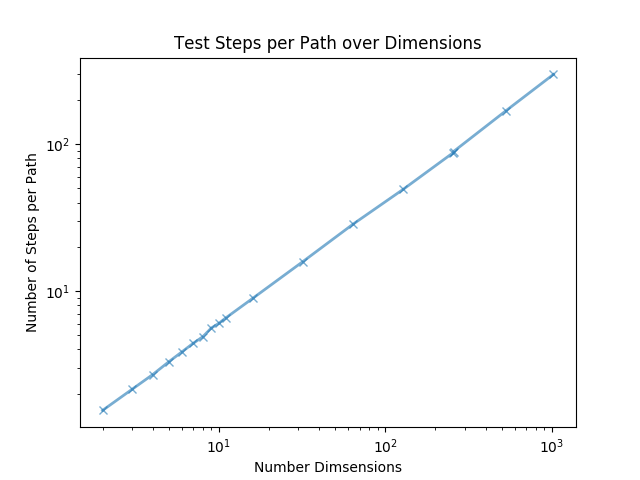
\includegraphics[width=10.0cm]{styles/pathsPerDim} \label{plot:pathsPerDim}
  \caption{Average number of steps per path sampled over a number of dimension}
\end{center}
\end{figure}
The linear regression of the above plot has a function of $$f(dimension)= 4.8108001661116715 + 0.2953577483675905*dimension.$$
A further point of interest is whether the number of steps per path remains smaller
than the period of the random number generator, namely $2^{190}$ or $~1.5 * 10^{57}$.
Each thread has its own seed, therefore the number of random numbers generated per
thread is of interest.  This number is equal to
$$maxRand = total Paths \% 65535 * f(dimension)$$ and is constrained by
$$ maxRand \overset{!}{<} 2^{190}$$
%TODO: table for f dimension.

%TODO: use largest possible value and find maximum

\section{Accuracy and Error}
In order to test the convergence and accuracy of this \Gls{RWoS} on \Glspl{GPU} implementation,
the exact solution for a two dimensional case was attained via a Fourie series in
two dimensions \cite{Bornemann}.  The resulting value is  $$u(0,0) = 0.29468 54131 26055 26226$$.
This value will be used as a known solution in order to check accuracy and convergence.
The plot bellow shows the convergence of the two dimensional case.


\section{Scaling Tests}
As with many programs, it was of interest to investigate the scaling properties of
of this \Gls{RWoS} program in respect to iterations and dimensions. From the theory,
we expect to see a scaling behavior that $\mathcal{O}( N\log(N))$ in nature.
%TODO: only power 2 dimensions
The hyper linear increase in running time is most likely due to the transition from
block based path iteration scaling to loop based iteration scaling once the maximum
number of blocks has been reached.  Since the block loops are executed in serial,
and dependencies limit the optimizations between loops.
\section{Speedup}
One of the main goals of this project was to show the possibility of decreasing computation
time of \Gls{RWoS} by running the algorithm on \Glspl{GPU}.  To show the resulting
speed increase, we will compare a CPU version of \Gls{RWoS} to the \Gls{GPU} version
created through this project.  Though such comparisons are sometimes frowned
upon, and called "misleading" due to the difference in underlying processor architecture,
the goal of this work was to show the computational acceleration, regardless of architecture.
The examples provided below represents an arbitrary sample, but serves to show the
computational acceleration possible through \Glspl{GPU}.  As a base-line \Gls{CPU}
reference performance number, an implementation of \Gls{RWoS} in the language
Julia will be used.  Julia provides a high level interface to highly optimized
numerical programming.  The author also provides a version of \Gls{RWoS} written
in C++, but this version lacks numerical optimization and is therefore slower than
the Julia base line.  Therefore, the Julia version is used, in order to provide
the most conservative \Gls{speed-up} numbers possible.
\par
The data below goes to show that the super linear speed up of high dimensional
\Gls{RWoS} on \Glspl{GPU} confirms the presumption that high dimensional problems
are well suited for \Glspl{GPU}.  Thanks to light context switches, large dimensional capabilities,
and the optimized \Gls{GPU} memory architecture and approach, the \Gls{GPU} implementation
of \Gls{RWoS} performs very well.

	 \label{part:thirdP}


	 % ---------------------------------------------------------------------------
	 %
	 % Appendix
	 %
	 % ---------------------------------------------------------------------------

	 \part*{Appendix}
	 \addcontentsline{toc}{part}{Appendix}

	 \appendix %---------------------------------------

	 \chapter{Detailed Descriptions}
%\section{Detailed Validation Results}
\label{chapter:DetailedDescriptions}\label{appendix}
Here come the details that are not supposed to be in the regular text.





 \clearemptydoublepage

 \printglossaries



 \bibliography{bibliography/literature}


\end{document}
